\documentclass[../Elmag-labhefte-2020.tex]{subfiles}


\begin{document}

\chapter{SIKKERHET I LABORATORIET \label{ch.elektrisitet} }


\vspace{1.5cm}


Eksperimentene i dette laboratoriekurset er sikre og medfører ingen fare dersom fornuftige og opplagte forholdsregler følges og studentene følger sikkerhetsinstruksjonene som gis nedenfor. Det eksisterer alltid en potensiell fare for elektrisk støt eller brann overalt hvor det finnes vegguttak, stikkontakter, kabling eller tilkoblinger, som finnes i alle laboratorier og hjem. Formålet med dette kapitlet  er å gi deg generell informasjon som skal forberede deg til å utføre laboratorieforsøk uten å sette deg selv eller andre i unødvendig fare, og å beskrive prosedyren som skal følges dersom du eller noen andre i nærheten befinner seg i en nødsituasjon.

%**********************************************
\section{Det elektriske utstyret}
%**********************************************



Som det fremgår av Ohms lov, $V = RI$, og loven om effektutvikling i en motstand, $P = VI = RI^2$, vil det alltid være et spenningsfall $V$ over en strømførende leder med strøm $I$ og motstand $R$, og det vil også alltid utvikles varme i lederen (forutsatt at $R > 0$).
 

For å sikre forbrukeren mot strømstøt, koples ytterkappen til alt utstyr som har ledende ytterkappe permanent til jord. Dette gjøres gjennom  jordingskontakten i støpselen. Dersom det oppstår feil som medfører at tilførselsspenningen til utstyret kommer i kontakt med den ledende ytterkappen, vil sikkerhetsjordingen sørge for at spenningen koples til jord og ikke legges på ytterkappen, med de farer dette innebærer. Strømmen vil altså kortsluttes til jord og normalt vil sikringen gå og strømmen brytes.\footnote{Det er i den forbindelse viktig at sikkerhetsjordledningen er dimensjonert slik at den tåler strømmen i hovedtilførselsledningen, dvs.\ den må minst ha samme tverrsnitt som hovedtilførselsledningen.}

For å unngå at personsikkerheten skal være avhengig av strømsikringene, utstyres elektriske energinett ofte med en såkalt \emph{nullstrømbryter}. Nullstrømbryteren kan oppdage jordlekkasjestrømmer som er mye mindre en kursens sikringsverdi. Dette gjør bryteren ved å sammenligne strømmen i de to ledningene til en kurs, dvs.\ strømmen inn til en forbruker med strømmen i retur fra forbrukeren. Tap av strøm hos forbrukeren tolkes som lekkasjestrøm til jord. Hvis nullstrømbryteren oppdager en forskjell mellom fase\-strømmene som er større enn en bestemt forhåndsinnstilt verdi (f.eks. \SI{30}{\milli\ampere}), så brytes strømmen. 

En tredje metode for å sikre forbrukeren mot strømstøt er \emph{dobbelt isolering} av utstyr (utstyr i klasse II, merket med en dobbeltfirkant:
\begin{picture}(12,12)
    \put(0,0){\line(1,0){10} }
    \put(10,0){\line(0,1){10} }
    \put(10,10){\line(-1,0){10} }
    \put(0,10){\line(0,-1){10} }
    \put(2,2){\line(1,0){6} }
    \put(8,2){\line(0,1){6} }
    \put(8,8){\line(-1,0){6} }
    \put(2,8){\line(0,-1){6} }
\end{picture}
\!). Dobbeltisolert utstyr må ikke forsøkes jordes da det vil redusere berøringssikkerheten.

Erfaring har vist at de aller fleste av feilene i elektriske anlegg er jordingsfeil. Vettug omgang med jord og korrekt jording av elektrisk utstyr er en forutsetning for trygg bruk av elektrisk energi og for at elektrisk utstyr virker korrekt. Plugg aldri elektrisk utstyr som krever jordet støpsel i en ikke-jordet stikkontakt.



%%%%%%%%%%%%%%%%%%%%%%%%%%%%%%%%
\section{Oppkopling av elektriske kretser}
%%%%%%%%%%%%%%%%%%%%%%%%%%%%%%%%

Ifølge Elektrisitetstilsynets forskrifter må alle vekselspenninger over \SI{25}{\V} effektivverdi og alle rippelfrie likespenninger over \SI{60}{\V} være forskriftsmessig isolert. Når du kopler opp kretser i laboratoriet, må du påse at disse forskrifter blir fulgt. 

Du må også passe på at ledningtverrsnittet til de ledninger du bruker er tilstrekkelig stort for at ledningene ikke blir opphetet. Selv om motstanden i elektriske ledninger er liten, vil ikke verdien alltid være neglisjerbar. For tvinnede kobberledninger som brukes til faste installasjoner i hus (med 230~V) sier forskriftene at en ledning med tverrsnitt \SI{2,5}{\mm\squared} maksimalt kan føre en strøm på \SI{16}{\ampere}. Som en tommelfingerregel i laboratoriet kan vi anta at \SI{5}{\ampere/\square\mm} ved spenninger under \SI{300}{\V} vil være trygt. De fleksible lissene vi bruker for oppkoplinger har alle tverrsnitt som er større enn \SI{1}{\square\mm}. Strømmer opp til \SI{5}{\ampere} vil derfor ikke by på noe problem for disse lissene. Et annet forhold du må passe på er å velge stort nok tverrsnitt på ledningene dine slik at spenningsfallet over ledningene ikke gir bidrag til målefeil.

Vær forsiktig med å sende strøm gjennom kveiler/tromler med elektrisk ledning. Grense\-kravene beskrevet over gjelder ledninger i friluft med naturlig luftavkjøling. Dersom ledningen kveiles tett sammen, vil varmeutviklingen føre til betydelig større temperaturøkning som kan føre til at isolasjonen kan smelte.

Når du bruker elektrisk koplingsmateriell er det viktig at du forsikrer deg om at alt materiell er i orden. Se etter skader på ledninger og spesielt kontakter. Det er også viktig at du behandler koplingsmateriellet slik at det ikke oppstår skader på det. Pass på å plassere ledningene under bruk slik at det ikke er fare for at de blir hektet fast i bevegelige deler eller kommer i klemme slik at isolasjonen skades. Ledningene bør også ligge fritt slik at de får tilstrekkelig avkjøling. Når ledningsmateriellet ikke er i bruk skal det ikke tvinnes opp da kraftig opptvinning kan skade isolasjonen og tilkoplingen mellom leder og kontakt. 


%%%%%%%%%%%%%%%%%%%%%%%%%%%%%%%%
\section{Innflytelse av elektriske strømmer på kroppen}
%%%%%%%%%%%%%%%%%%%%%%%%%%%%%%%%

Faren ved elektriske støt er forbundet med størrelsen på den strømmen som går gjennom kroppen og hvilken strømbane den følger. Hvor stor spenning kroppen tåler vil avhenge av den totale motstanden i strømkretsen hvor kroppen inngår. Figur \ref{fig:Kroppen} viser menneskekroppen som en del av en strømkrets.


\begin{figure}[htbp] 
    \centering
    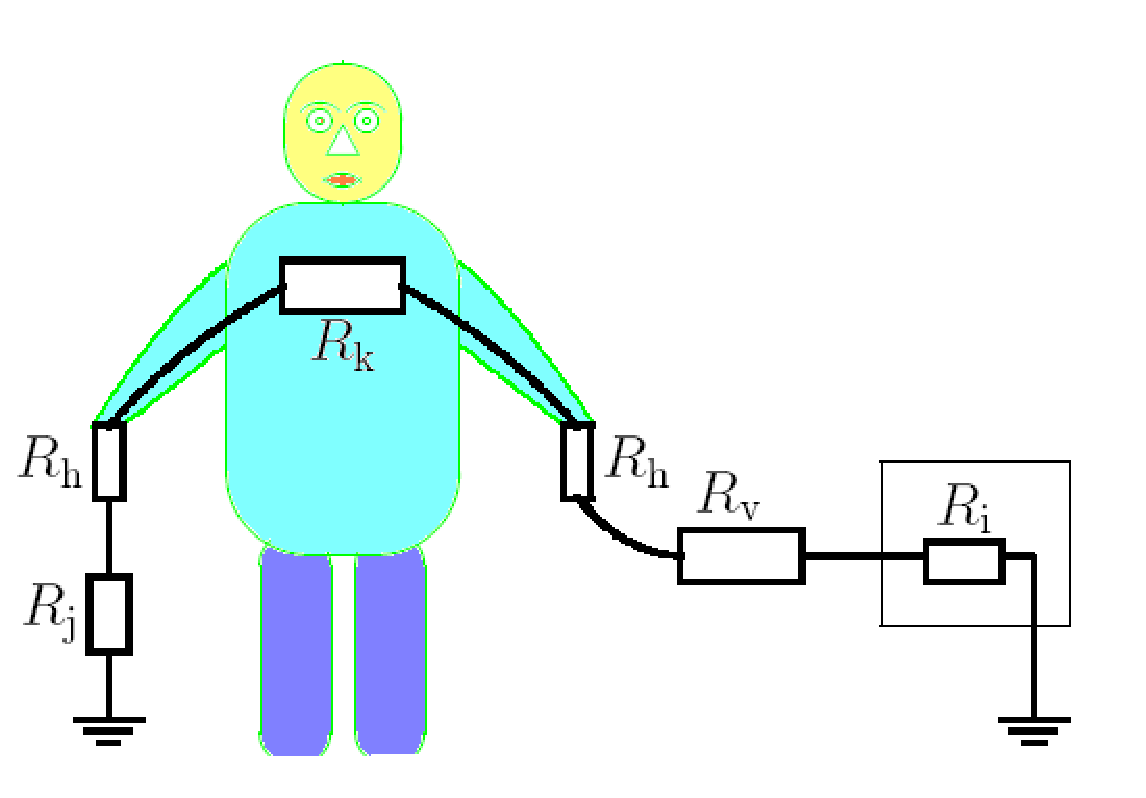
\includegraphics[width=10cm,height=6.96cm,keepaspectratio]{Kroppen_resized}
    \caption{
    Menneskekroppen som del av en strømkrets, hvor $R_\text{j}$ er isolasjonsmotstanden mellom kroppen og jord, $R_\text{h}$ er overgangsmotstanden i huden, $R_\text{k}$ er kroppens indre motstand, $R_\text{i}$ er indre motstand i spenningskilden som driver strømmen i kretsen og $R_\text{v}$ er isolasjonsmotstanden mellom spenningskildens spenningsterminal og kroppen.
    }
    \label{fig:Kroppen}
\end{figure}

Strømgjennomgang kan skade kroppen, enten ved at den skader kroppsvevet ved oppvarming, eller ved at strømmen forstyrrer de elektriske signalene i nervesystemet. Oppvarmingen er gitt av strømmen $I$ og motstanden $R$ i vevet som varmes opp. En vedvarende strøm gjennom vevet over tid vil tilføre en stadig større varmeenergi og risiko for skade. Forstyrrelse av de elektriske signalene i nervesystemet kan bl.a.\ føre til hjerteflimmer og lammelser. Spesielt er vekselstrøm i frekvensområdet \num{15} til \SI{60}{\hertz} farlig for nervesystemet. Vår nettforsyning på \SI{50}{\hertz} er derfor i den farlige kategorien. Når frekvensen på vekselstrømmen øker, vil innflytelsen på nervesystemet avta, og for frekvenser over \SI{10}{\kilo\hertz} er innflytelsen tilnærmet borte. Oppvarmingseffekten er imidlertid fremdeles til stede. 

Strømbaner gjennom hjerte- og lungeregionen er spesielt farlige pga.\ de vitale organene som der finnes. Nyrene er også spesielt følsomme for strømskader. 

Fra strømkretsen i figur \ref{fig:Kroppen} ser vi at strømmen gjennom kroppen er gitt ved 

\begin{equation}
    I = \frac{V}{R_\text{j} + 2R_\text{h} + R_\text{k} + R_\text{i} + R_\text{v}}.
    \label{eq:BodyVoltDiv}
\end{equation}

Når det blir referert til spenningen på et forsyningsnett menes vanligvis effektivverdien av spenningen, definert som

\begin{equation}
    V_\text{eff}
        = \sqrt{\langle V(t)^2 \rangle}
        = \sqrt{\frac{1}{T} \int_0^T V_0^2 \sin^2 \qty(\frac{2\pi t}{T}) \dd{t}}
        = \frac{V_0}{\sqrt{2}}.
    \label{eq:EffectiveV}
\end{equation}

Det betyr at for et \num{230} volts anlegg er toppspenningen (amplituden) $V_0 = \sqrt{2} \times \SI{230}{\V} = \SI{325}{\V}$.

Sikkerhetstiltak mot strøm går ut på å redusere verdien på strømmen gjennom kroppen til ufarlige verdier. Dette kan for en gitt spenning $V$ gjøres ved å sørge for at summen av motstandene under brøkstreken er tilstrekkelig stor:

\begin{itemize}
    \item[$R_\text{v}$] Vanlig elektrisk isolasjon av elektrisk utstyr går ut på å gjøre $R_\text{v}$ tilstrekkelig stor. 
    
%    \item[$R_\text{i}$] I laboppgaven i kapittel \ref{ch.coulomb} bruker du en \SI{12000}{\V} høyspenningskanon. Den blir ufarliggjort ved å gjøre $R_\text{i}$ så stor at $V/R_\text{i} < \SI{0,5}{\milli\ampere}$. 
    
    \item[$R_\text{k}$] Kroppens indre motstand $R_\text{k}$ er konstant og av størrelsesorden \SI{500}{\ohm}. Legg merke til at grensen for påbudt isolasjon av vekselspenning på \SI{25}{\V} effektiv spenning tilsvarer \SI{50}{\milli\ampere} når vi antar at motstanden i strømkretsen kun består av kroppens indre motstand, dvs.\ verste tilfelle.
    \item[$R_\text{h}$] Overgangsmotstanden $R_\text{h}$ i huden kan variere fra \SI{0}{\ohm} ved fuktig hud til langt over \SI{10000}{\ohm} ved tørr hud. $R_\text{h}$ avtar også med økende spenning og den varierer også med frekvensen slik at den er lavest i frekvensområdet rundt \SI{50}{\hertz}. Dette medvirker til å gjøre vekselspenning farligere enn likespenning. Et annet forhold som gjør vekselspenning farligere enn likespenning er at størrelsen på spenningen det refereres til når vekselspenning omtales er effektivspenningen. Toppspenningen er imidlertid $\sqrt{2} \times $ høyere, som beskrevet i likning \eqref{eq:EffectiveV}.
    \item[$R_\text{j}$] Dersom kroppen ikke er i kontakt med jord, vil $R_\text{j}$ være stor.  Hvorfor dør ikke fuglene når de sitter på kraftledninger (se figur \ref{fig:BirdA})? Svar på dette spørsmålet ved å modifisere figur \ref{fig:Kroppen}. Se nå på figur \ref{fig:BirdB}, og svar så på spørsmålet stilt der.
    %Fugler som setter seg på høyspenningslinjer tar ikke skade p.g.a.\ at $R_{\rm j}$ er stor. Hvis handa di er i kontakt med en vannkran eller jordet ledning er $R_{\rm j} \approx 0 \; \Omega$.
\end{itemize}

\begin{figure}[!ht]
    \begin{minipage}[b]{0.49\linewidth}
        \centering
        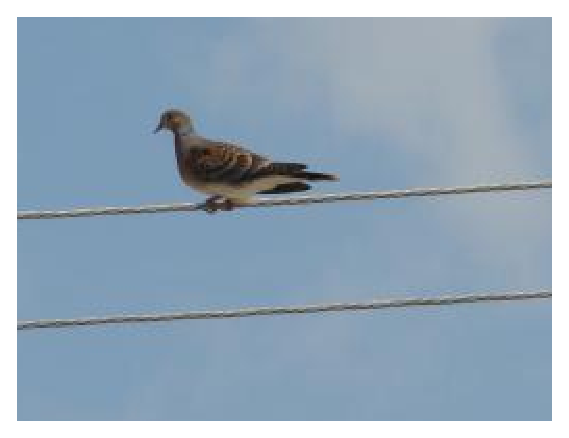
\includegraphics[scale=0.82]{fig/BirdL.eps}
        \caption{%
            En fugl som sitter på en kraftlinje.
        }
        \label{fig:BirdA}
    \end{minipage}
    \hspace{0.1cm}
    \begin{minipage}[b]{0.49\linewidth}
        \centering
        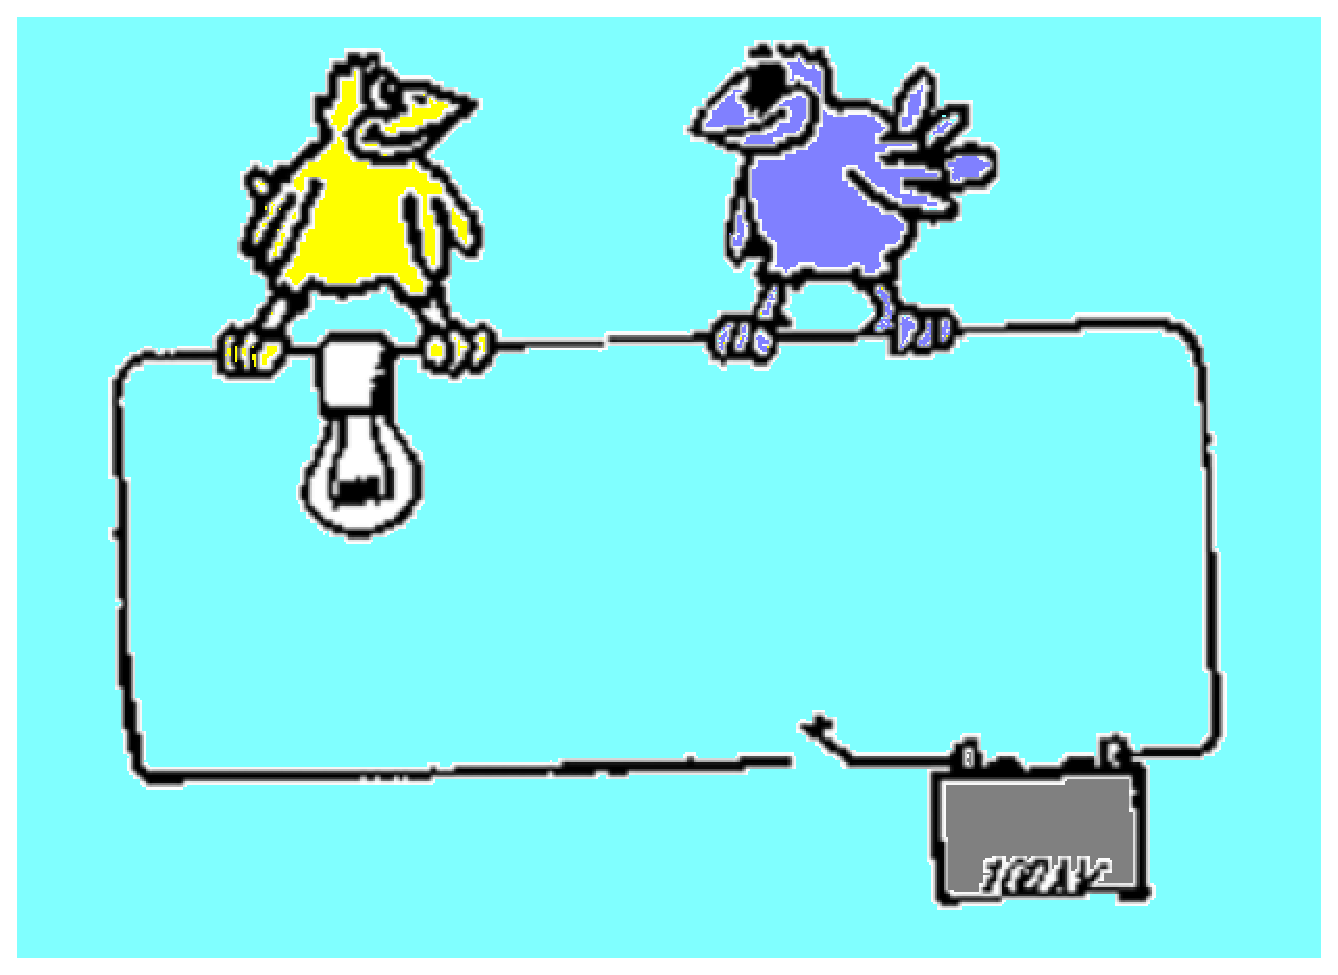
\includegraphics[scale=0.35]{fig/BirdC.eps}
        \caption{%
            Hva skjer når den slås på?
        }
        \label{fig:BirdB}
    \end{minipage}
\end{figure}

I tillegg til ovenstående er det viktig å være klar over at høyfrekvent elektromagnetisk stråling i \si{\mega\hertz}--\si{\giga\hertz}-området (mikrobølger--radar) kan være farlig for kroppen ved at det elektriske vekselfeltet fører til oppvarming av kroppsvevet, samme effekt som gir oppvarming i en mikrobølgeovn. Slik høyfrekvent oppvarming er ekstra farlig fordi den ofte foregår uten at normale smertefunksjoner trer i kraft. Personer bør skjermes hvis effekt per flateenhet mot kroppen er $> \SI{0,01}{\watt/\cm\squared}$. 

\begin{table}[!ht]
    \begin{center}
    \caption{Limits of exposure\textsuperscript{a} to static magnetic fields}
    \label{tab:exposurlimits}
        \begin{tabular}{ l  c  c }
        \hline
        \noalign{\bigskip}
        \qquad\qquad Exposure characteristics &  & Magnetic flux density  \\
        \noalign{\medskip}
        \hline
        \noalign{\medskip}
        Occupational\textsuperscript{b} &  &  \\ 
        \noalign{\smallskip}
            \quad Exposure of head and trunk&   &  \SI{2}{\tesla} \\ 
            \quad Exposure of limbs\textsuperscript{c} & &  \SI{8}{\tesla}\\
        \noalign{\medskip}
        General public\textsuperscript{d} &  &  \\ 
        \quad Exposure of any part of the body& & \SI{400}{\milli\tesla}\\
        \noalign{\medskip}
        \hline
        \noalign{\medskip}
        \end{tabular}
    \end{center}
    \vspace*{-0.7cm}
\end{table}
%
\begin{figure}[!ht]
    \centering
    \begin{minipage}[t]{0.7\textwidth}
    \footnotesize{
        \textsuperscript{a} ICNIRP recommends that these limits should be viewed operationally as spatial peak exposure limits.\\
        \textsuperscript{b} For specific work applications, exposure up to \SI{8}{\tesla} can be justified, if the environment is controlled and appropriate work practices are implemented to control movement-induced effects.\\
        \textsuperscript{c} Not enough information is available on which to base exposure limits beyond \SI{8}{\tesla}.\\
        \textsuperscript{d} Because of potential indirect adverse effects, ICNIRP recognizes that practical policies need to be implemented to prevent inadvertent harmful exposure of persons with implanted electronic medical devices and implants containing ferromagnetic material, and dangers from flying objects, which can lead to much lower restriction levels such as \SI[output-decimal-marker = {.}]{0.5}{\milli\tesla}.
    }
    \end{minipage}
\end{figure} 


%%%%%%%%%%%%%%%%%%%%%%%%%%%%%%%%
\section{Virkning av statisk magnetfelt}
%%%%%%%%%%%%%%%%%%%%%%%%%%%%%%%%
Den internasjonale kommisjon for beskyttelse mot ikke-ioniserende stråling (ICNIRP) gir i sine retningslinjer anbefalte grenseverdier for eksponering for elektromagnetiske felt (se tabell \ref{tab:exposurlimits}). I Norge er det i strålevernforskriften gitt bestemmelser om at ICNIRPs retningslinjer skal følges, og at all eksponering skal holdes så lavt som praktisk mulig. For statisk magnetfelt er anbefalt grense \SI{2}{\tesla} for arbeidstakere og \SI{400}{\milli\tesla} for generell befolkning. Personer med pacemaker, ferromagnetiske implantater eller implanterte elektroniske komponenter bør ikke utsettes for magnetfelt over \SI{0,5}{\milli\tesla}.\footnote{\url{http://www.icnirp.de/documents/emfgdl.pdf} [\textit{Health Physics} \textbf{96} (2009) 504--519.]} I eksperimentet der Helmholtzspolene brukes vil den magnetiske flukstettheten $B$ i umiddelbar nærhet av spolene ha en verdi som så vidt overstiger \SI{0,5}{\milli\tesla} for $I = \SI{1}{\ampere}$ og $R = \SI{0,07}{\m}$, hvor $I$ er strømmen som flyter i spolene og $R$ er den gjennomsnittlige radien til spolene. Men feltet avtar raskt utenfor spolene; størrelsen av $B$ i et punkt vinkelrett på spolen i avstand \SI{0,15}{\m} (eller større) fra spolens sentrum er mindre enn \SI{50}{\micro\tesla}. Dersom en strømstyrke på \SI{0,5}{\ampere} brukes, vil feltet overalt være lavere enn anbefalt grense for personer med implantater. En student med et implantat som er følsomt for magnetfelt bør informere ansvarspersonen, som vil sørge for at denne studenten har en partner som ikke har implantat og at partneren gjør målingene.


%%%%%%%%%%%%%%%%%%%%%%%%%%%%%%%%
\section{Sunn fornuft i omgang med elektrisk utstyr}
%%%%%%%%%%%%%%%%%%%%%%%%%%%%%%%%

I tillegg til de vanlige risikoene i forbindelse med elektrisitet, har noen laboratorier høyspenningsutstyr\footnote{For vår hensikt vil det være nok å betrakte enhver spenning høyere enn \SI{50}{\V} som høyspenning.} som utgjør en enda større potensiell fare. Studenter bør være ekstra forsiktige med slikt utstyr, og bør lære seg hvordan de kan frakoble strømkilden i en nødssituasjon. Her er noen regler som må følges når man arbeider med og i nærheten av elektrisitet. 

\begin{enumerate}
    \item Ikke arbeid med elektrisitet dersom dine hender, føtter, eller andre deler av kroppen er våte, eller hvis du står på et vått gulv.
    \item Inspiser elektrisk utstyr (med strømmen avslått og stikkontakten trukket ut) for ødelagte ledninger og skadede tilkoblinger. Hvis noe slikt oppdages, ikke bruk utstyret. Meld så i fra til ansvarshavende slik at utstyret kan repareres.
    \item Forsøk aldri å reparere elektrisk utstyr selv---dette må gjøres av kvalifisert personell. 
    \item Dersom du blir utsatt for selv et mildt støt fra noe utstyr, lever det umiddelbart inn til reparasjon.
    \item Ikke bruk eller lagre ekstremt brannfarlige væsker i nærheten av elektrisk utstyr. Noen stoffer, slik som eter, kan antennes av gnist fra elektrisk utstyr. 
    \item Bruk alltid jordede stikkontakter i jordede vegguttak. Forsøk aldri å sette en jordet stikkontakt inn i et ujordet vegguttak.
    \item Skjøteledninger bør ikke brukes i stedet for permanent kabling; de bør kun brukes midlertidig og de bør ikke trekkes under dører, på tvers av ganger, gjennom vinduer eller hull i vegger, rundt rør eller i nærheten av vasker.
    \item Ikke overbelast kretser ved å bruke grenuttak på ett vanlig uttak.
    \item Ikke fjern eller endre på sikkerhetstiltak på høyspenningsutstyr. Husk at de er der for å beskytte deg.
    \item Vær sikker på at strømmen er slått av under tilkobling eller når endringer på kretsen foretas.
    \item Vær sikker på at alt utstyr er satt med riktige innstillinger iht. målingen som skal utføres før kretsen gjøres strømførende.
    \item Vær sikker på at komponentene som brukes er av en gradering som kan motstå pålagt strøm og spenning.
    \item Erstatt ødelagte sikringer med nye av riktig type og med korrekte spesifikasjoner.
    \item {\itsf Hvis du tror noen har vært utsatt for et kraftig elektrisk sjokk\/}:
    \begin{itemize} 
        \item ikke fjern den skadede fra den elektriske kilden før strømmen har blitt slått av.
        \item hvis du ikke får slått av strømmen, bruk noe isolerende slik som et tørt tau, klut eller kosthåndtak for å dra personen bort fra strømmen.
        \item sjekk om det er kontakt.
        \item sjekk om det er pust.
        \item sikre frie luftveier.
        \item når skadde ikke puster eller ved hjertestans, ring 113 AMK-sentralen.
        \item gi hjerte-/lungeredning (HLR) 30 kompresjoner og 2 innblåsninger. Fortsett til helsepersonell kommer.
        \item puster den skadde selv, legges personen i stabilt sideleie.
        \item let etter brannskader og kjøl ned brannsår med vann og behandle dem som tredjegradsforbrenning.
        \item alle skadde skal ha tilsyn etter at førstehjelp er gitt. Ikke forlat bevisstløse personer. Bevisste personer skal snakkes med. Personskader skal behandles videre av medisinsk personell.
        \item personer som sendes til Legevakten i drosje/privatbil skal følges helt fram og inn. Ta med evt. HMS-datablad!
        \item alle ulykker/tilløp til ulykker er å betrakte som avvik i forhold til normal drift, og skal meldes på avviksskjema.
    \end{itemize}
\end{enumerate}

I forsøket med Coulombs lov, gir høyspenningskanonen som brukes for å lade opp kulene \SI{25}{\kilo\V} når den aktiveres. Strømmen er imidlertid begrenset til \SI{75}{\micro\ampere}. Slike strømmer har vanligvis ingen fysiologisk virkning på kroppen, men likevel: \textit{Behandle kanonen som om den var livsfarlig}.

\end{document}
